\subsection{Dafny Specific Features}\label{dffeatures}
This chapter details the language specific features that were implemented during the project. Since Dafny focuses on an elegant way of writing specification constructs, the goal of these features is to aid the programmer writing them. While such constructs have great potential helping to write correct code, most programmers are not yet used to thinking in terms of this methodology. Additionally, there are situations which appear often that warrant the writing of similar specification constructs. While important, this work can become tedious. The features detailed in this chapter try to mitigate both these points. \newline
\subsubsection{Counter Examples}
\paragraph{What are Counter Examples}
Dafny's proof pipeline works by trying to find a proof by contradiction. This means, that when a programmer writes a specification construct such as a postcondition, Dafny and its pipeline try to find a situation where the postcondition does not hold. If no violation is found, the proof obligation is satisfied. \newline
If however, a violation is found, that means that the pipeline has found a set of assignments to the variables involved in the context of the postcondition that led to the postcondition being violated. The set of such assignments that lead to a violation is called a counter example. \newline
Counter examples are split up into different states. This means, Dafny includes all assignments to each variable in each state of control flow in a context. This may seem very abstract, but it becomes clear when shown in a simple example. \newline
\begin{figure}[H]
	\centering
	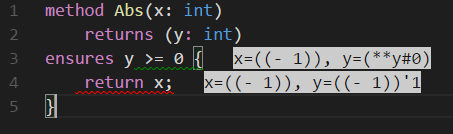
\includegraphics[width=1\textwidth]{img/counterModel}
	\caption{Counter Example is shown in Visual Studio Code}
	\label{fig:dfcounterModel}
\end{figure}
When a counter example is generated for a postcondition of a method as seen in \ref{fig:dfcounterModel}, Dafny determines the value of each variable at each point of execution. In the example, there is only one line of code in the method body. This means that the method has two states. The first one is before the line is executed, in this case, only the parameter x is set to a value which will lead the postcondition to be violated. The return value y has not been set yet, so the counter model at this state does not yet hold a value for y. \newline
At the next state of computation, the line in the method body has been evaluated. Dafny's counter model no not only shows the value of x, but also the value of y which can be determined after that line of code has been evaluated. \newline
In summation, a counter model shows the values of all variables involved at all stages of computation that lead to a specification construct being violated. 
\paragraph{Why where they chosen to implement}
To widen the circle of Dafny programmers, it is important to support Dafny specific features in a language integration. Displaying counter example was chosen mainly because of two reasons. The first one is that many programmers are not used to writing specification constructs, so displaying counter examples is a good way to clarify what a specification constructs actually expresses, deepening the understanding of the programmer. \newline
The second consideration is that edge cases are a continuous source of errors. While they may often be forgotten when writing specification constructs, they are most likely the values that Dafny finds to build a counter model with. This quickly leads to the inclusion of edge cases when thinking of error free code, something which is difficult to achieve for IDEs. \newline
A more internal notion on why they were integrated is that, as detailed in \ref{evaluation}, the project failed to deliver a generic approach towards contract generation. Displaying counter examples is a way to partly make up for this missing feature, as it supports the programmer finding correct constructs. 
\paragraph{What benefits do they entail}
Counter examples greatly deepen the understanding of code, as they bring to attention possible situations that the programmer did not think of. When writing complex code, it is nearly impossible to have all possible contexts in mind that it can run and possibly fail in. The displacement of counter examples helps the programmer reasoning on when implementations satisfy specification constructs, which is ultimately the main goal behind the design of Dafny. \newline
They also help writing correct specification constructs, which is not always easy. When constantly being shown counter examples on when a contract is violated, the programmer can refine a contract iteratively until it is no longer violated. This is also the approach that most modern proofing frameworks follow. \newline
\begin{figure}[H]
	\centering
	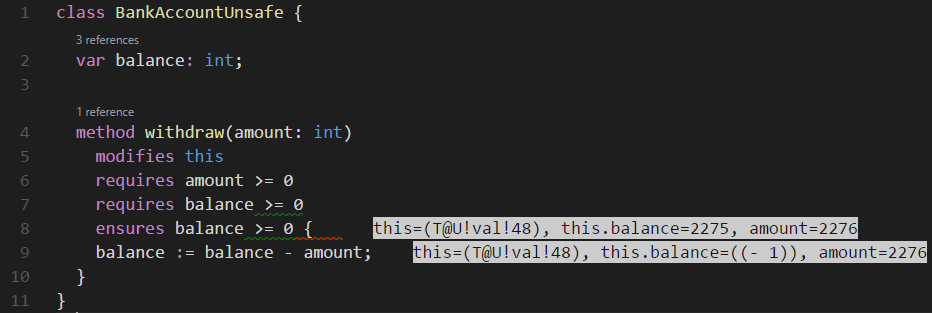
\includegraphics[width=1\textwidth]{img/counterModelBank}
	\caption{Complex Counter Example with multiple specifications}
	\label{fig:dfcounterModelBank}
\end{figure}
As already detailed in the paragraph above, counter examples also often show edge cases that lead to a condition not being satisfied, a very important consideration when programming. These can then easily be taken care of appropriately by the programmer, either by changing the specification construct or the implementation. Without displaying this information, it is very difficult for the programmer to exactly find out how a condition is violated. \newline
This project is the only solution that displays counter examples except for the Visual Studio integration, a feature which is probably the most important Dafny specific aid an IDE can provide. 
\subsubsection{Null Checks}
\paragraph{What are Null Checks}
Null checks are specification constructs that take the form of a precondition that requires an object to be not null. They can be written whenever a new context is opened. Examples are when an object is given as an argument to a method, then the specification is a precondition to the whole method. Another one is when a object is declared, potentially not initialized and used in a later following while block. Then the precondition is written for the while block.\newline
\begin{figure}[H]
	\centering
	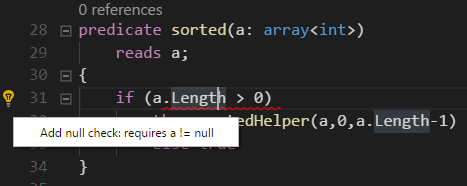
\includegraphics[width=0.7\textwidth]{img/nullCheck}
	\caption{A situation that profits from a Null Check}
	\label{fig:dfnullcheck}
\end{figure}
When a null check is written in form of such a precondition, the following context can safely interact with the object, since it is sure that the object is initialized. 
\paragraph{Why were they chosen to implement}
Programmers very often access members of elements, especially in the methodology of object oriented programming. While it offers a great way to structure a program and to represent reality in a program, it comes with some danger. The most common pitfall usually is the null reference. To help avoid this, Dafny reports potential null references. Since almost any piece of complex code deals with objects, this is a very common occurrence, since for instance every object given as an argument must be checked for null first. \newline
It was therefore decided to offer a mitigation of this important, but tedious work. The insertion of such a precondition shifts the burden of providing valid arguments to the caller of a context, so the implementation can concentrate on providing functionality. While working with Dafny, it was noticed that such a precondition was needed for about every third method, and every other while block, meaning that a lot of work is done for the programmer by supplying this precondition generation.
\newline
Providing this Dafny specific feature was implemented as the first code fix, since a null reference arguably is the most common trivial error when programming in the object oriented methodology. Offering an automated solution to this in an IDE makes Dafny's strengths shine and working with it more enjoyable.
\paragraph{What benefits do they entail}
Current solution do not support the automatic generation of null checks, something which occurs very often when programming. Avoiding null references is important, but tedious work. Providing an automated fix for this enables the programmer to work in a safe context and to concentrate on providing functionality without having to think about checking the context first. \newline
\begin{figure}[H]
	\centering
	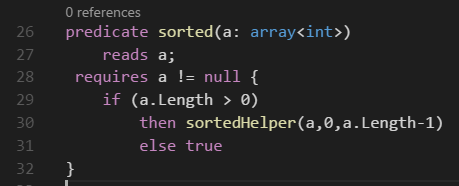
\includegraphics[width=0.7\textwidth]{img/nullCheckApplied}
	\caption{An example of a Null Check}
	\label{fig:dfnullcheckapplied}
\end{figure}
This improves productivity, since it narrows the problems that the programmer has to deal with himself. Providing null checking therefore helps the programmer writing code more quickly and profit from Dafny in an automated way.
\subsubsection{Bound Checks}
\paragraph{What are Bound Checks}
When accessing an array, this is done by providing an expression that is used as an index into that array. Since an array has a fixed length, it is important that the expression resolves to a value inside the array's range. \newline
\begin{figure}[H]
	\centering
	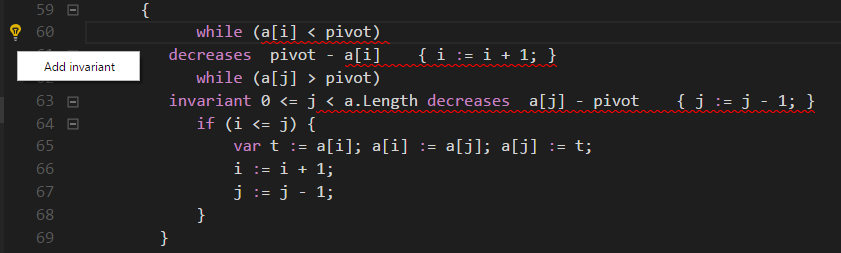
\includegraphics[width=1\textwidth]{img/indexOutRangeDiag}
	\caption{Accessing an array without making sure the index is in bound}
	\label{fig:dfindexOutOfRange}
\end{figure}
Since the definition of an array's range is always the set of integers between zero and the array's length minus one, bound checks can be implemented as two specification constructs that take the form of preconditions belonging to the context in which the array is accessed in. \newline
The first precondition states that the expression used as an index must resolve to a value bigger or equal to zero, the second one that the expression must resolve to a value smaller than the array's length. When these two preconditions hold, it is sure that the array access will succeed and not result into a memory violation. 
\paragraph{Why where they chosen to implement}
Since Dafny has enough knowledge about the array data structure, it issues compilation errors every time an array is accessed without checking for its bounds first. While programming with Dafny, it was observed that this is the case in almost every non trivial example using arrays. Since the array data structure is used quite often in Dafny, it was decided to also help the programmer with this construct, since bound checking is important, but tedious.
\paragraph{What benefits do they entail}
Current solution do not support the automatic generation of bound checking. This task has to be performed very often and is tedious. Relieving the programmer of this repetitive work frees his mind for working on core functionality of a product. \newline
\begin{figure}[H]
	\centering
	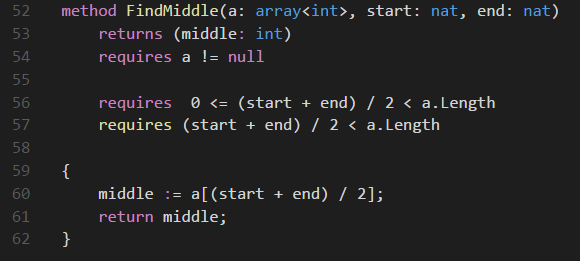
\includegraphics[width=1\textwidth]{img/boundCheck}
	\caption{Bound checks were generated}
	\label{fig:dfindexInBound}
\end{figure}
Automatically resolving these checks therefor makes working with Dafny more efficient and is part of making the plugin more usable and supportive.
\subsubsection{Increase / Decrease / Invariant Guards}
\paragraph{What are they}
These constructs that are called guards in this paper help ensuring that an expression complies with certain conditions. This is done by writing specification constructs that ensure this. 
\newline
In case of increase or decrease guards, this is done by either writing an increase or a decrease specification construct, demanding that an expression either increases or decreases. This is often needed to meet loop termination or when using recursion, in both cases Dafny recognizes that an expression should change over time in a certain way and requires constructs detailing this. This makes sure that for instance recursion reaches a termination clause or a loop terminates. \newline
\begin{figure}[H]
	\centering
	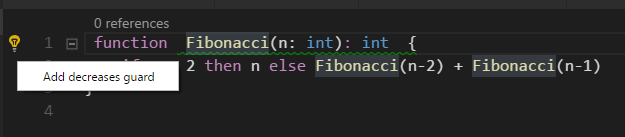
\includegraphics[width=0.7\textwidth]{img/decreaseGuard}
	\caption{Recursion should always decrease an expression}
	\label{fig:dfdecreaseguard}
\end{figure}
In case of invariants, it is done by writing a specification construct called an invariant. When an expression used in an invariant can be dynamic, it specifies to which range of values it can resolve. 
This is for instance needed when an expression used as an index to an array is dynamic inside of a loop. The invariant then makes sure that the expression is always in bound of the array. 
\paragraph{Why were they chosen to implement}
The first two guards are needed to  make sure an expression converges to a certain range of values over time. This is the case when making use of recursion to ensure that the base case is eventually met, or when writing loops that depend on a certain value of an expression for termination. Both examples are very important, because not handling them correctly can result in endless loops or overflow. Dafny already does a good job in generating warnings that tell the programmer that constraints should be enforced for a certain expression. These situations also occur very often, since both recursion and loops are fundamental elements of programming.\newline
Often, an expression must always evaluate into a certain range, this is for instance the case when an expression that is used as an index to an array is not constant within the context of a loop. \newline
Since the above detailed constructs are used often, and the appropriate specification constraints help using them correctly, it was decided to implement an automatic way of generating them. 
\paragraph{What benefits do they entail}
No existing solution offers an automatic way of generating these guards, a tasks which soon was discovered was tedious and time consuming, because it is not always clear at first glance which expressions are subject to constraints. Providing an automatic way of generating them does ensure that the specification constructs are declared correctly, manually inserting them is error prone and demands some reasoning by the programmer.  \newline
\begin{figure}[H]
	\centering
	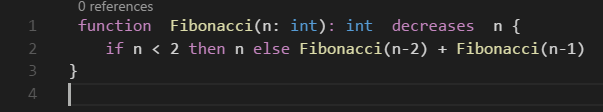
\includegraphics[width=0.7\textwidth]{img/decreaseGuardApplied}
	\caption{Recursion guided by a decrease guard}
	\label{fig:dfdecreaseguardapplied}
\end{figure}
This feature therefor allows the programmer to be more productive and concentrate on key areas of concern.
\subsubsection{Flow Graphs}
\paragraph{What are they}
A existing feature in Boogie is to translate boogie programs into a flow graph. It does not only show the flow of the program itself but also includes all pre- and postconditions. Below is an example of a flowgraph, taken from the partition method of a quicksort algorithm.\newline  
\begin{figure}[H]
	\centering
	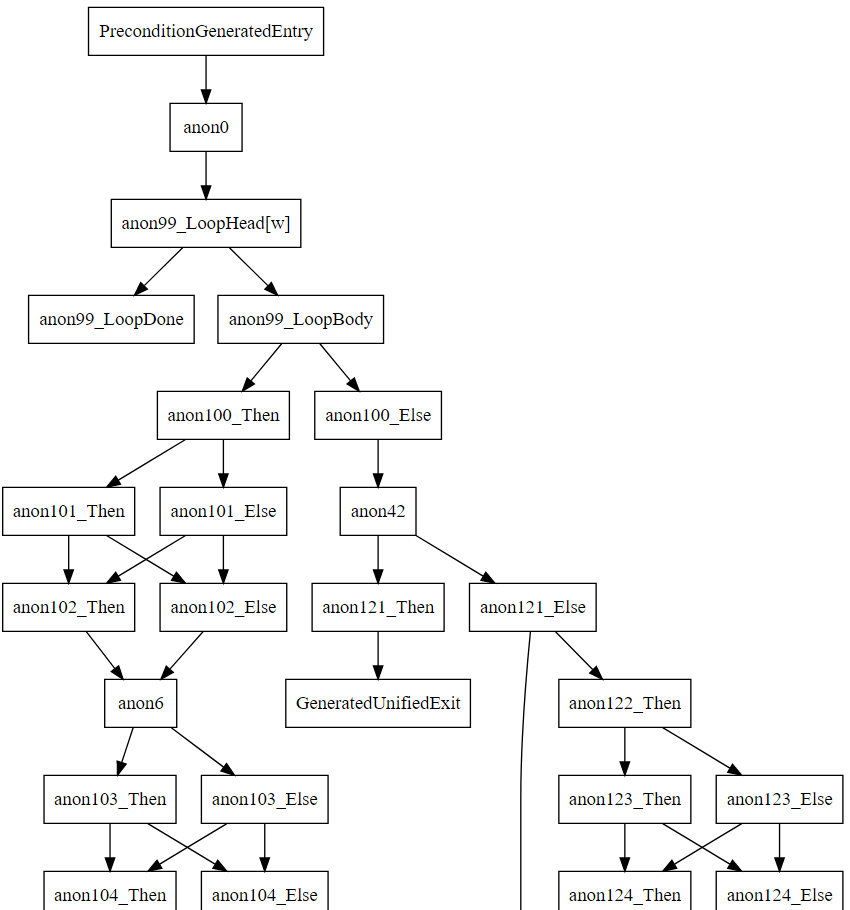
\includegraphics[width=1.0\textwidth]{img/flowgraph}
	\caption{Flow Graph of the partition method}
	\label{fig:flowgraph}
\end{figure}
\paragraph{Why were they chosen to implement}
Because this feature existed already in Boogie, and the goal was to support as many features from the Dafny pipeline as possible, it was decided that this feature could be easily and nicely implemented. 
\paragraph{What benefits do they entail}
Developers can directly see the flow of the program they are working on in Visual Studio Code. Otherwise, they would need to manually save the graph to a file, upload or convert the file to finally view it. This all is done in the background to provide a nice user experience.
